\documentclass[11pt]{article}

\usepackage[backend=biber,style=mla]{biblatex}
\usepackage[margin=1in]{geometry}
\usepackage[utf8]{inputenc}
\usepackage{setspace}
\usepackage{amsmath}
\usepackage{amssymb}
\usepackage{mathtools}
\usepackage{esint}
\usepackage{titlesec}
\usepackage{graphicx}
\usepackage{wrapfig}
\usepackage{blindtext}
\usepackage{fancyhdr}

\addbibresource{/home/krttd/Documents/UAH.bib}

\doublespacing

\pagestyle{fancy}
\lhead{}
\chead{}
\cfoot{}
\rhead{Dodson \thepage}

\renewcommand*{\bibfont}{\normalsize}

\titleformat{\section}
{\large}{}{0em}{}[\titlerule]


\begin{document}

\begin{singlespace}
Mitchell Dodson

Dr. Ryan Weber % Professor

EH 301 % class

Ferbruary 18, 2020 % date
\end{singlespace}

\begin{center}
{\Large\sc
How to write comprehensions in Python
}
\end{center}

% The Python language's tasteful inclusion of syntactic sugar including lambda operators, inline logic, and comprehensions solidify the language's dominance for both scripting and production programming, however these strategies may seem arbitrary and esoteric at first.

\begin{center}
Python comprehensions offer a quick and visually intuitive (but initially somewhat esoteric) method for creating and restructuring iterable objects such as tuples, dictonaries, and lists.
\end{center}


\begin{center}
	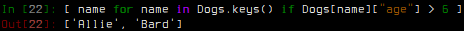
\includegraphics[width=.66\linewidth]{./figures/comp.png}
	\label{comp} %(to reference in the future text)
\end{center}

\noindent
\begin{minipage}[h]{.67\textwidth}
	The example we will use (pictured above) supposes we want a list of the names of dogs older than 6, and refers to the ``Dogs''dictionary (defined in the image to the right).
	\begin{enumerate}
		\item{Decide what data type you want your comprehension to create. In the example, the output will be a \emph{list}, denoted by the square brackets surrounding the definition}
		\item{Pick the item that you want to compose your new list with as well as the existing iterable from which you will derive the new list. in the example, we want to make a list of the dogs' names, which are the keys of the Dogs dictionary. Use the \textbf{in} operator to specify the parent iterable.}
		\newcounter{enumTemp}
		\setcounter{enumTemp}{\theenumi}
	\end{enumerate}
\end{minipage}
\begin{minipage}[h]{.33\textwidth}
	\hfill
	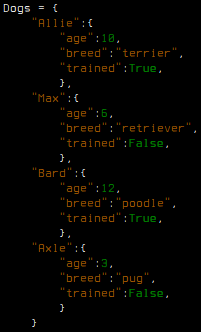
\includegraphics[width=.8\linewidth]{./figures/dict.png}
	\label{dict} %(to reference in the future text)
\end{minipage}

\begin{enumerate}
	\setcounter{enumi}{\theenumTemp}
	\item{Apply a constraint to narrow down the items that get included in the output list. In our example, we use an \textbf{if} statement to only select dogs whoge age is over 6}
	\item{If you only want to include items \emph{derived} from the members of the parent iterabel (as shown below), you can modify the selector to modify the selected item}
\end{enumerate}

\vfill
\begin{center}
	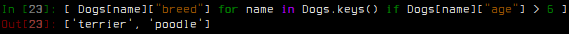
\includegraphics[width=.75\linewidth]{./figures/comp2.png}
	\label{comp2} %(to reference in the future text)
\end{center}

If used correctly, the interpreter will return a new iterable with the specified items. Comprehensions are ultimately clear and easy-to-use but powerful operators; enjoy your ability to find new and creative ways to implement them!



\printbibliography
\end{document}
